
\section{Sphärische Trigonometrie}
In der sphärischen Trigonometrie gibt es eine Symetrie zwischen Seiten und Winkel, also zu jedem Satz über Seiten und Winkel gibt es einen entsprechenden Satz, mit dem man Winkel durch Seiten und Seiten durch Winkel ersetzt hat.
Dabei gibt es folgenden Zusammenhang zwischen der ebenen- und sphärischen Trigonometrie:

\subsection{Das Kugeldreieck}
Damit man die Definition des Kugeldreiecks versteht, müssen wir zuerst Begriffe wie "Grosskreisebene" und "Grosskreisbögen" verstehen.
Ein Grosskreis ist ein größtmöglicher Kreis auf einer Kugeloberfläche.
Sein Mittelpunkt fällt immer mit dem Mittelpunkt der Kugel zusammen und ein Schnitt auf dem Großkreis teilt die Kugel in jedem Fall in zwei gleich grosse Hälften.
Da es unendlich viele Möglichkeiten gibt, eine Kugel so zu zerschneiden, dass die Schnittebene den Kugelmittelpunkt trifft, gibt es auch unendlich viele Grosskreise.
Grosskreisbögen sind die Verbindungslinien zwischen zwei Punkten auf der Kugel, welche auch "Seiten" eines Kugeldreiecks gennant werden.

Werden drei voneinander verschiedene Punkte, die sich nicht auf derselben Grosskreisebene befinden, mit Grosskreisbögen verbunden, so entsteht ein Kugeldreieck $ABC$.
Für ein Kugeldreieck gilt, dass die Summe der drei Seiten kleiner als $2\pi$ aber grösser als 0 ist.
$A$, $B$ und $C$ sind die Ecken des Dreiecks und dessen Seiten sind die Grosskreisbögen zwischen den Eckpunkten (siehe Abbildung 21.2). 

Da die Länge der Grosskreisbögen wegen der Abhängigkeit vom Kugelradius ungeeignet ist, wird die Grösse einer Seite mit dem zugehörigen Mittelpunktwinkel des Grosskreisbogens angegeben. 
Laut dieser Definition ist die Seite $c$ der Winkel $AMB$, wobei der Punkt $M$ die Erdmitte ist.

Man kann bei Kugeldreiecken nicht so einfach unterscheiden, was Innen oder Aussen ist. 
Wenn man drei Eckpunkte miteinander verbindet, ergeben sich immer 16 Kugeldreiecke. 
Jenes Kugeldreieck mit den Seitenlängen $a, b, c < \pi$ und den Winkeln $\alpha, \beta, \gamma < \pi$ nennt man Eulersches Dreieck.

Es gibt einen Zusammenhang zwischen der ebenen- und sphärischen Trigonometrie, wobei folgend $a$ eine Seite beschreibt:
\begin{center}
	\begin{tabular}{ccc}
		Eben & $\leftrightarrow$ & sphärisch \\
		\hline
		$a$ & $\leftrightarrow$  & $\sin \ a$  \\
		
		$a^2$ & $\leftrightarrow$  & $-\cos \ a$ \\
	\end{tabular}
\end{center}

\begin{figure}
	\begin{center}
		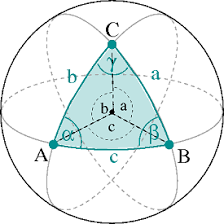
\includegraphics[width=6cm]{papers/nav/bilder/kugel1.png}
		\caption[Das Kugeldreieck]{Das Kugeldreieck}
	\end{center}
	
\end{figure}

\subsection{Rechtwinkliges Dreieck und rechtseitiges Dreieck}
Wie auch im ebenen Dreieck gibt es beim Kugeldreieck auch ein rechtwinkliges Kugeldreieck, bei dem ein Winkel $\frac{\pi}{2}$ ist. 
Ein Rechtseitiges Dreieck gibt es jedoch nur beim Kugeldreieck, weil dort eine Seitenlänge $\frac{\pi}{2}$ lang sein muss.
\begin{figure}
	
	\begin{center}
		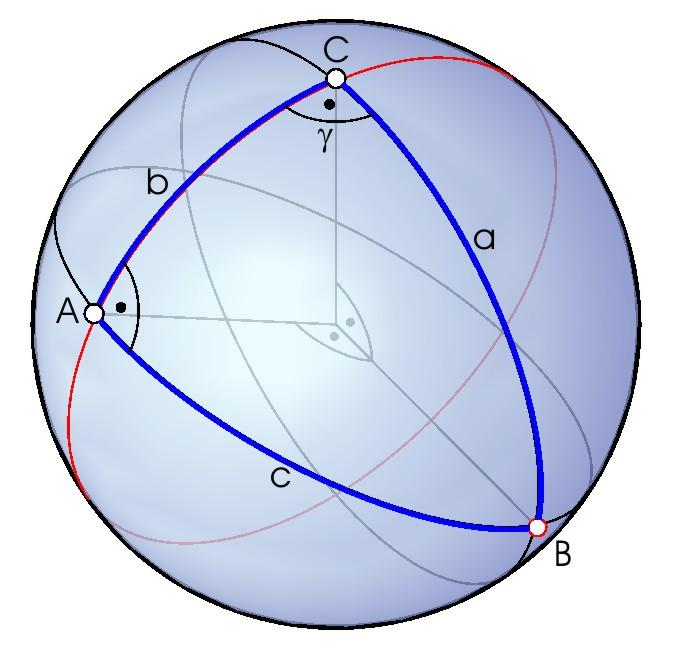
\includegraphics[width=10cm]{papers/nav/bilder/recht.jpg}
		\caption[Rechtseitiges Kugeldreieck]{Rechtseitiges Kugeldreieck}
	\end{center}	
\end{figure}

\subsection{Winkelsumme}
\begin{figure}
	
	\begin{center}
		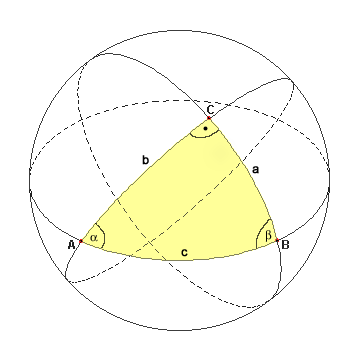
\includegraphics[width=8cm]{papers/nav/bilder/kugel2.png}
		\caption[Winkelangabe im Kugeldreieck]{Winkelangabe im Kugeldreieck}
	\end{center}	
\end{figure}


Die Winkel eines Kugeldreiecks sind die, welche die Halbtangenten in den Eckpunkten einschliessen. 
Für die Summe der Innenwinkel gilt
\begin{align}
	\alpha+\beta+\gamma &= \frac{F}{r^2} + \pi \ \text{und} \ \alpha+\beta+\gamma > \pi, \nonumber
\end{align}
wobei F der Flächeninhalt des Kugeldreiecks ist.
\subsubsection{Sphärischer Exzess}
Der sphärische Exzess
\begin{align}
	\epsilon = \alpha+\beta+\gamma - \pi \nonumber
\end{align}  
beschreibt die Abweichung der Innenwinkelsumme von $\pi$ und ist proportional zum Flächeninhalt des Kugeldreiecks.

\subsubsection{Flächeninnhalt}
Mithilfe des Radius $r$ und dem sphärischen Exzess $\epsilon$ gilt für den Flächeninhalt 
\[ F=\frac{\pi \cdot r^2}{\frac{\pi}{2}} \cdot \epsilon\].
\subsection{Sphärischer Sinussatz}
In jedem Dreieck ist das Verhältnis des Sinus einer Seite zum Sinus des Gegenwinkels konstant. 
Das bedeutet, dass

\begin{align}
	\frac{\sin (a)}{\sin (\alpha)} =\frac{\sin (b)}{\sin (\beta)} = \frac{\sin (c)}{\sin (\gamma)} \nonumber
\end{align}
auch beim Kugeldreieck gilt.

\subsection{Sphärische Kosinussätze}
Auch in der sphärischen Trigonometrie gibt es den Seitenkosinussatz
\begin{align}
	\cos \ a = \cos b \cdot \cos c + \sin b \cdot \sin c \cdot \cos \alpha \nonumber
\end{align} %Seitenkosinussatz
und den Winkelkosinussatz

\begin{align}
	\cos \gamma = -\cos \alpha \cdot \cos \beta + \sin \alpha \cdot \sin \beta \cdot \cos c. \nonumber
\end{align}

\subsection{Sphärischer Satz des Pythagoras für das rechtwinklige Kugeldreieck}
Es gibt in der sphärischen Trigonometrie eigentlich garkeinen "Satz des Pythagoras", wie man ihn aus der zweidimensionalen Geometrie kennt.
In der sphärischen Trigonometrie gibt es aber auch einen Satz, der alle drei Seiten eines rechtwinkligen Kugeldreiecks, nicht aber für das rechtseitige Kugeldreieck, in eine Beziehung bringt. 
Es gilt nämlich:
\begin{align}
	\cos c = \cos a \cdot \cos b \ \text{wenn} \nonumber &
	\alpha = \frac{\pi}{2} \nonumber
\end{align}
 